In a introductory stats class, would calculate statistics like \underline{sample mean} or \underline{sample standard deviation} from data $x_i$ where $i$ indexes observations $i=1,...,n$ 
\begin{align*}
    \bar{x}&=\frac{1}{n}\sum_{i=1}^n x_i \\
    \hat{\sigma}&=\sqrt{\frac{1}{n}\sum_{i=1}^n (x_i - \bar{x})^2}
\end{align*}
Instead, in a time series describe \underline{types of variation}:
\begin{itemize}
    \item Seasonal variation
    \item Cyclical variation
    \item Trend
    \item Size of other irregular fluctuations
\end{itemize}

\underline{Trend}: 
\begin{itemize}
    \item[] Suppose data is denoted $x_1,...,x_t,...,x_T$ where:
    \begin{itemize}[label=\textbullet]
        \item $T$ is the length of the time series
        \item $t$ indexes time
        \item $x$ is a general variable to denote values
        \item $x_t$ is a value at time $t$
    \end{itemize}
\end{itemize}
$X_t = \alpha + \beta t + \varepsilon_t$, where $\varepsilon_t$ are irregular and "no trend" (later defined Stationarity) then $X_t$ has a linear trend with slope $\beta$



First, basic notation

A time series is denoted $\{X_t\}_{t=1}^T$
\begin{itemize}
    \item $x$ is the variable observed
    \item $x_t$ is the value at time $t$
    \item $T$ is the length of the time series
    \item $X_t$ is a sequence of random variables $\Rightarrow$ Calculating mean or variance of $X_t$ possible
\end{itemize}

Breaking up a time series into components
\begin{itemize}
    \item[] There are several types of components you might try to decompose a time series into
    \begin{itemize}
        \item Deterministic Trend
        \item Seasonal or Cyclical variation
        \item Stationary component
    \end{itemize}
\end{itemize}

\subsection{Formal Definition of Stationary Time Series}

\begin{mdframed}
A time series $\{X_t\}$ is \underline{strictly stationary} if for any positive integer $k$ and $n$-tuple of positive integers $(t_1,t_2,...,t_n)$ the joint distribution function of $(X_t, X_{t_2},...,X_{t_n})$ equals the joint distribution function of $(X_{t+k}, X_{t_2+k}, ..., X_{t_n+k})$
\end{mdframed}
Intuitively, the time series "looks the same" in terms of its randomness at all points in time.

Example:

\[ \text{Let }\Tilde{x}_t = 
\begin{cases} 
0 & \text{if day t's coin flip is heads}, \\
1 & \text{if day t's coin flip is tails}.
\end{cases}
\]
This is stationary.

Example:

\[ \text{Let }x_t = 
\begin{cases} 
0 & \text{if day t's coin flip is heads}, \\
1 & \text{if day t's coin flip is tails}. \\
\end{cases}
\]
except: \quad every time there are 3 heads in a row, do not toss a coin, but make the next point tails. If $\Tilde{x}_{t-3}=\Tilde{x}_{t-2}=\Tilde{x}_{t-1}=$ heads then assign $\Tilde{x}_t=$ tails.

\begin{itemize}
    \item[] \underline{Property}
    \begin{itemize}
        \item[] If $X_t$ and $Y_t$ are time series and they are independent from each other and $X_t$, $Y_t$ are stationary, then $X_t + Y_t$ is stationary
    \end{itemize}
    \item \underline{Property}
        \begin{itemize}
            \item[] If $X_t$ is stationary, then $X_t - X_{t-1}$ is stationary
        \end{itemize}
\end{itemize}

\subsection{Trends in Time Series}


Trend is a term usually reserved for slow changes in the mean of a time series $X_t$

The simplest example of a time series with a trend is one of the form 
$$X_t = \alpha = \beta t + \varepsilon_t$$
where \begin{itemize}
    \item $\alpha$ and $\beta$ are real numbers
    \item $\varepsilon$ is stationary \underline{and} mean zero.
\end{itemize}
Sometimes, write $\mu_t = \alpha + \beta t$ and assume $E[\varepsilon_t]=0$. Call $\mu_t$ the mean of the time series. Because

\begin{align*}
    E[X_t] &= E[\alpha + \beta t + \varepsilon_t] \\
    &= E[\alpha + \beta t] + E[\varepsilon_t] \\
    &= \alpha + \beta t + 0\\
    &= \mu_t
\end{align*}

More general classes of trends:
\begin{itemize}
    \item Polynomial: 
    $$X_t=\alpha+\beta t +\gamma t^2 + \nabla t^3 + \varepsilon_t$$
    \item Geompertz trend:
    $$ X_t = \alpha exp(b\ exp(-ct)) + \varepsilon_t$$, $c>0$
    \item Exponential:
    $$X_t =a\ exp(bt) + \varepsilon_t$$
\end{itemize}
Models of Global trend: a small number of parameters captures information about the trend at all points in time.

Many ways to estimate and extract a global trend.

Example: \quad Least Squares:
\begin{adjustwidth}{2em}{0pt}
For a linear trend $X_t=\alpha + \beta t + \varepsilon_t$\
Estimate $(\hat{\alpha}, \hat{\beta})=\underset{a,b}{min} \frac{1}{T} \sum_{t=1}^T (X_t-a-bt)^2$
\end{adjustwidth}

$X_t =$ Trend$(X_t) + $res$(X_t)$
\begin{itemize}
    \item res$(X_t)=\hat{\varepsilon}_t=X_t-\hat{\alpha} -\hat{\beta}t $
    \item Trend$(X_t)=X_t-$ res$(X_t)$
    \item Both are estimates. If $\varepsilon_t$ is stationary and $T$ large enough, then $\hat{\alpha}+\hat{\beta}t \approx \alpha+\beta t$ with high probability
\end{itemize}

\begin{figure}[h]
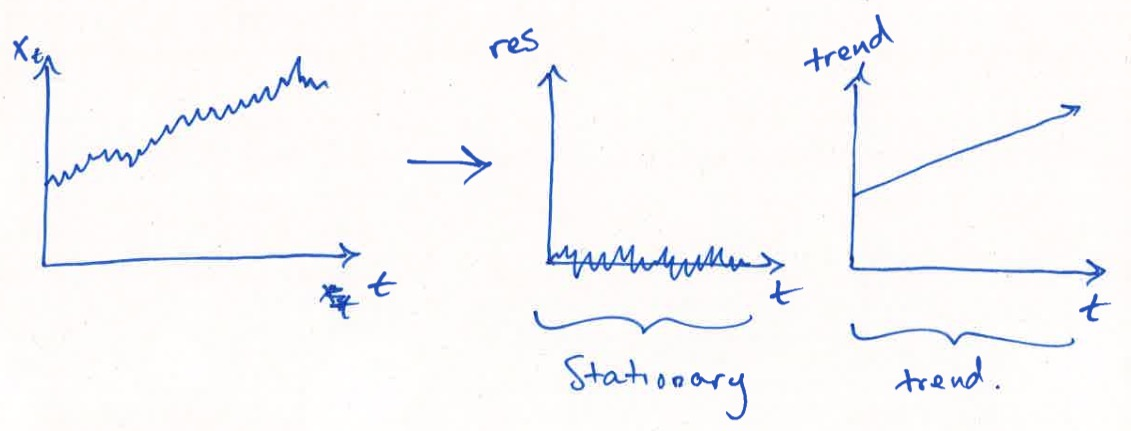
\includegraphics[scale=0.3]{images/Screenshot 2024-03-29 at 16.08.14.jpg}
\centering
\end{figure}

\subsubsection{Local Trend Extraction}



\textbf{Linear filtering}: Transform $X_t$ into $Y_t$ according to $$Y_t = \sum_{r=-q}^S a_rX_{t+r}$$

\begin{itemize}
    \item $\{a_r\}$ is a set of weights
    \item This operation is often called a moving average
\end{itemize}

Notation: \quad $Y_t=SM(X-t)$ \quad Sm="smoothed"

Examples of weight schemes:
\begin{itemize}
    \item Spencer's 15-point MA (moving average) with $q=7$:
    $$\{a_r\}=\frac{1}{320}(-3,-6,-5,3,27,46,67,74,67,...)$$
    \item Simple MA:
    $$a_r=\frac{1}{2q+1} \text{ for } r=-q,-q+1,...,q$$ 
\end{itemize}


\begin{figure}[h]
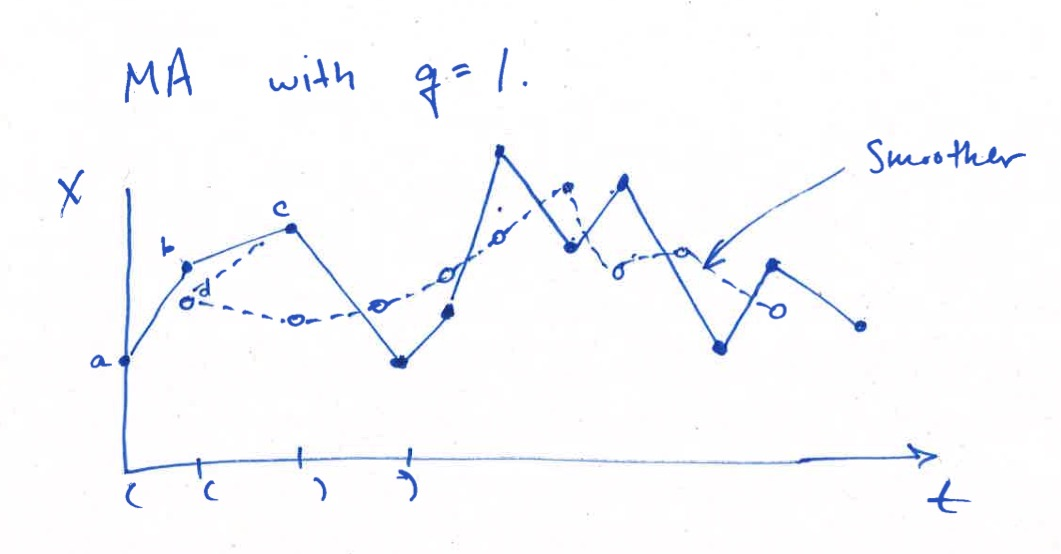
\includegraphics[scale=0.3]{images/Screenshot 2024-03-30 at 14.22.35.jpg}
\centering
\end{figure}


Again, like in Global trend extraction, for any linear filter, can calculate.
\begin{mdframed}
\centering
res$(X_t)=X_t-$ Sm$(X_t)$
\end{mdframed}

\bigskip

\textbf{End effect problem}

\bigskip
If observed $ \{X_t\}_{t=1}^T $ cannot smooth forward at $X_T$. With simple MA with $q=1$, $Sm(X_t)=\frac{1}{3}(X_{t-1}+X_t+X_{t+1})$. Cannot calculate $Sm(X_T)$. Don't know $X_{T+1}$.

Can use asymmetric filters:
$$Sm(X_t)=\sum_{r=-q}^0 a_r X_t$$
$\Rightarrow X_{t+1}$ never affects $Sm(X_t)$
\begin{itemize}
    \item Exponential Smoothing $Sm(X_t)=\sum_{j=0}^\infty a(1-a)^j x_{t-j}$
    \item First Difference average $Sm(X_t)=\frac{1}{2}(X_t+X_{t-1}$
\end{itemize}


\textbf{Differencing}:
\begin{itemize}
    \item $Y_t =X_t-X_{t-1} = \nabla X_t$ (first order differencing)
    \item $Z_t=\nabla Y_t= (X_t-X_{t-1})-(X_{t-1}-X_{t-2})=X_t-2X_{t-1}+X_{t-2}=\nabla^2X_t$ (Second order differencing)
\end{itemize}

\textbf{Kernel Smoothing}

\bigskip

Any type of smoothing where weights specified by a Kernel function. 
$$Sm(X_t)=\sum_{t'=1}^T w_t(t'), \quad w_t(t')= \frac{K\left(\frac{t-t'}{b} \right)}{\sum_{t''=1}^T K\left( \frac{t-t''}{b}\right)}$$

\begin{itemize}
    \item "Kernel function" $K$. \quad Example: $K(\cdot)=e^{\frac{-(\cdot)^2}{2}}$
    \item "Bandwidth b" number 
\end{itemize}

\bigskip

\underline{Sequential filtering (Convolution)}

\bigskip

\begin{itemize}
    \item First, filter $\{X_t\}$ with weights $\{a_r\}$ to obtain $\{y_t\}$
    \item Then, filter $\{y_t\}$ with weights $\{b_j\}$ to obtain $\{z_t\}$
    \item How to get the 'combined' weights $\{c_k\}$?
        \begin{itemize}
            \item We can compute:
            \[
            z_t=\sum_j b_j y_{t+j}=\sum_jb_j \sum_r a_r x_{t+j+r} = \sum_k c_k X_{t+k}, \quad \text{ where } c_k=\sum_r a_r b_{k-r}
            \]
        \end{itemize}
\end{itemize}

\subsubsection{Detrending a Time Series}

\begin{figure}[h]
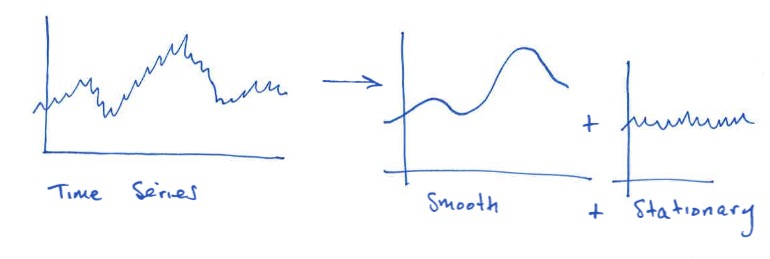
\includegraphics[scale=0.4]{images/Screenshot 2024-03-30 at 15.07.16.jpg}
\centering
\end{figure}

Globals approach was: use a parametric functional form, e.g., $X_t=\beta t+\varepsilon_t$, $\beta$ estimated via least squares

Local approach was: Smoothing, $Y_t=Sm(X_t)=\sum_r a_r X_{t-r}$

Can detrend Seasonality trends with local smoothing. E.g., number of Influenza cases recorded, seasonal because there is a predictable peak in winter.

Standard for Seasonality:
\begin{align*}
    Y_t=Sm(X_t)&=\frac{0.5 X_{t-6} + X_{t-5}+...+X_{t+5} + 0.5 X_{t+6}}{12}\\
    Res(X_t)&=X_t-Sm(X_t) \quad \text{$\Rightarrow$ num. of surprise cases}
\end{align*}

Other procedures are available too, used by e.g., US Census Bureau:
\begin{itemize}
    \item X12 ARIMA
    \item SEATS-TRAMO
    \item X13 ARIMA-SEATS
\end{itemize}

\subsection{Autocorrelation and the Correlogram}

Goal: Come up with a method for measuring dependence between observations across time.

\begin{itemize}
    \item Remember the definition of sample correlation of two random variables $\Romanbar{X}$ and $\Romanbar{Y}$ with data $(X_1,Y_1), ..., (X_T,Y_T)$
    \begin{align*}
        r&=\frac{\sum_{t=1}^T (X_t-\bar{X})(Y_t-\bar{Y})}{\sqrt{\sum_{t=1}^T (X_t-\bar{X})^2 \times \sum_{t=1}^T (Y_t-\bar{Y})^2}} \\
        \bar{X}&= \frac{1}{T} \sum_{t=1}^T X_t &&= \text{average}(\Romanbar{X}) \\
        \bar{Y} &= \frac{1}{T} \sum_{t=1}^T Y_t &&= \text{average}(\Romanbar{Y})
    \end{align*}
    \item What happens if $X_t=Y_t$? Then $r=1$
\end{itemize}

Apply correlation idea to lags of time series
\begin{itemize}
    \item For example, let $(X_t, Y_t)=(X_t, X_{t-1})$
    \item Warning: this only measures "linear dependence"
\end{itemize}


Carrying the idea out: 
Define:
\begin{align*}
        r&=\frac{\sum_{t=1}^{T-1} (X_t-\bar{X}_{(1)})(X_{t+1}-\bar{X}_{(2)})}{\sqrt{\sum_{t=1}^{T-1} (X_t-\bar{X}_{(1)})^2 \times \sum_{t=1}^{T-1} (X_{t+1}-\bar{X}_{(2)})^2}} \\
        \bar{X}_{(1)} &= \sum_{t=1}^{T-1} \frac{X_t}{T-1} \\
        \bar{X}_{(2)} &= \sum_{t=1}^{T-1} \frac{X_{t+1}}{T-1} 
\end{align*}

Most researchers use approximation $\bar{X}_{(1)} \approx \bar{X}_{(2)} \approx \bar{X} $ and terms in denominator are $\approx$. This gives 
$$r_1=\frac{\sum_{t=1}^{T-1} (X_t-\bar{X})(X_{t+1}-\bar{X})}{\sum_{t=1}^{T} (X_t-\bar{X})^2}$$

Terminology for r:
\begin{itemize}
    \item Sample autocorrelation of lag 1
    \item First order autocorrelation coefficient
    \item Usage of terminology is author dependent
\end{itemize}

Can do this for larger lags: \quad Let $k>0$ be an integer lag. Let 
$$r_k=\frac{\sum_{t=1}^{T-k} (X_t-\bar{X})(X_{t+k}-\bar{X})}{\sum_{t=1}^{T} (X_t-\bar{X})^2}$$

\begin{itemize}
    \item $k$-th order autocorrelation coefficient
    \item Caution: Really only used for stationary time series
\end{itemize}

\underline{Exc. 2.4 (Book)}: \quad With a truly random process (under the assumption of a Gaussian white noise process) it is expected that the sample autocorrelation coefficient fall inside the C.I. that is given as: $\pm z\times \sqrt{\frac{1}{N}}$. (Note: in a random process it is normal to find some coefficient to fall just outside the C.I.)


\textbf{\underline{Correlogram}}: \quad A plot of autocorrelation coefficients.

\begin{itemize}
    \item Choose a number $M<T$. E.g., if $T=200$, $M=30$ might be used
\end{itemize}

\begin{lstlisting}[language=R]
# In R (status package)
acf(x)        #(uses M=10*log_10(T))
                #(Horizontal bounds at +- 2/\sqrt(T) )
\end{lstlisting}

Example:

\begin{figure}[h]
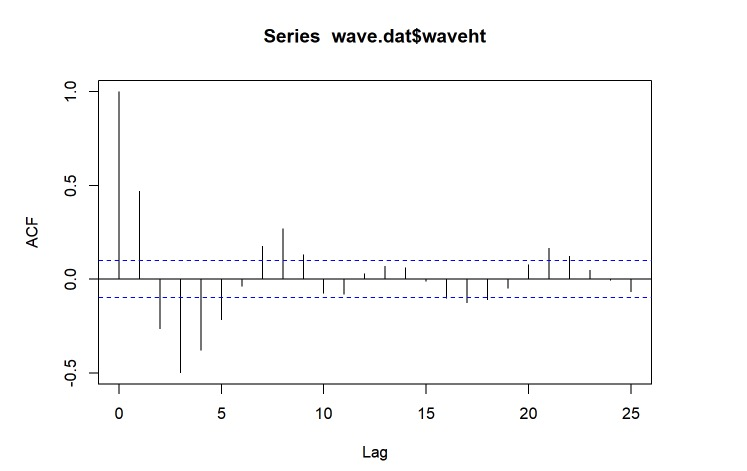
\includegraphics[scale=0.4]{images/Screenshot 2024-03-30 at 17.42.36.jpg}
\centering
\end{figure}


\subsection{Transformations}

In many cases, to reduce the unwanted effects of outliers of statistical routines can apply transformations to a time series

Example:

\begin{figure}[htbp]
  \centering
  \begin{minipage}{0.49\textwidth}
    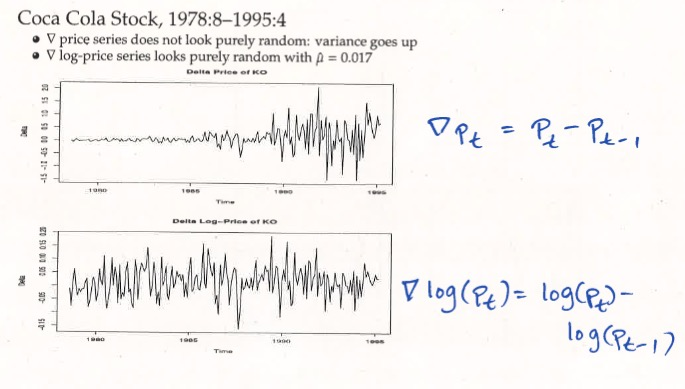
\includegraphics[height=5cm]{images/Screenshot 2024-03-30 at 17.45.04.jpg} % Left image
  \end{minipage}\hfill
  \begin{minipage}{0.49\textwidth}
    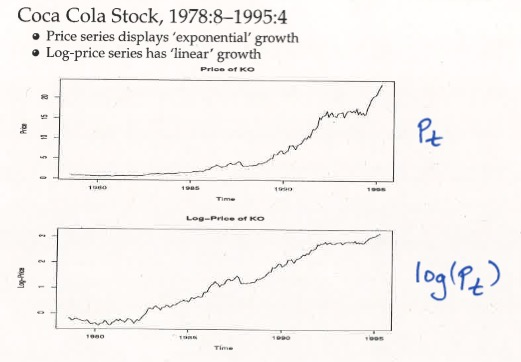
\includegraphics[height=5cm]{images/Screenshot 2024-03-30 at 17.46.58.jpg} % Right image
  \end{minipage}
\end{figure}



